\documentclass{article}
\usepackage{amsmath}
\usepackage{amssymb}
\usepackage{xcolor}
\usepackage{amsthm}
\usepackage{dsfont}
\usepackage{graphicx}
\usepackage{hyperref}
\usepackage{datetime}
\usepackage{todonotes}
\usepackage[noend]{algpseudocode}
\usepackage{algorithm}
\usepackage{tikz}

\renewcommand\algorithmicthen{}
\renewcommand\algorithmicdo{}
\renewcommand{\algorithmicrequire}{\textbf{Input:}}


% inline comments
% you could use \listoftodos to print an overview
\newcommand{\inline}[1]{ {\color{blue}{#1}}\addcontentsline{tdo}{todo}{#1}}
\newcommand{\comment}[1]{{\color{blue}\noindent{#1}\\}\addcontentsline{tdo}{todo}{#1}}
% use this one to disable
%\newcommand{\inline}[1]{\ignorespaces}


\newdateformat{monthyeardate}{\monthname[\THEMONTH] \THEYEAR}

\newcommand{\newmarkedtheorem}[1]{%
  \newenvironment{#1}
    {\pushQED{\qed}\csname inner@#1\endcsname}
    {\popQED\csname endinner@#1\endcsname}%
  \newtheorem{inner@#1}%
}

\theoremstyle{definition}
%\newtheorem{eg}{Example}[section]
\newmarkedtheorem{eg}{Example}[section]
\newtheorem{observation}{Observation}[section]
\newtheorem{remark}{Remark}
\theoremstyle{plain}
\newtheorem{define}{Definition}
\newtheorem{proposition}{Proposition}
\newtheorem{theorem}{Theorem}[section]
\newtheorem{assump}{Assumption}


\title{Network with Finite Buffers}
\author{Jeroen van Riel}
\date{\monthyeardate\today}

\begin{document}

\section*{Bounded lane capacity}

Up to this point, we have not taken into account the fact that lanes between
intersection have finite capacity. We need to incorporate this aspect in order
to develop a model that could be used for practical applications. Under high
traffic loads, lanes with finite buffer capacity can prevent vehicles from
crossing upstream intersections. Therefore, the traffic controller needs to take
into account these additional constraints.

\begin{figure}[h]
  \centering
  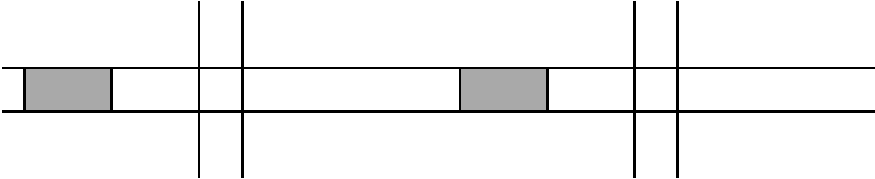
\includegraphics[width=0.7\textwidth]{figures/tandem.pdf}
  \caption{Illustration of two intersections in tandem.}\label{fig:tandem}
\end{figure}

% First, rewrite MotionSynthesize more compactly, using state variables z(t) =
% (x(t), \dot{x}(t)).
% Next, write the checkpoint constraints.


We start with the simplest extension of the single intersection model by
considering two intersections in tandem, as illustrated in Figure~\ref{fig:tandem}. Let the
$v$ denote the left intersection and $w$ the right intersection and assume that
traffic drives from left to right. Let the length and width of vehicle $i$ be
denoted by $L_{i}$ and $W_{i}$, respectively. We measure the position of a
vehicle at the front bumper and we let position $x=0$ be at the stopline of
intersection $v$. Let the position of intersection's $w$ stopline be denoted by
$x=d(v,w)$. To simplify the following discussion, we make the following
assumption on the vehicle sizes.
\begin{assump}
  All vehicles have the same length $L_{i} = L$ and width
  $W_{i} = W$.
\end{assump}

First, we investigate the trajectories generated by the
\texttt{MotionSynthesize} procedure and derive crossing time constraints that
are sufficient to maintain safety.
%
The minimum time required for a vehicle to come to a full stop or, equivalently,
to accelerate to full speed from a stop, is given by
\begin{align*}
  \hat{t} = \frac{v_{\max}}{a_{\max}} .
\end{align*}
The trajectory of full stop is given by
\begin{align*}
  x(t) = \frac{t^{2} a_{\max}}{2} ,
\end{align*}
so the minimum distance required for a vehicle to fully accelerate or decelerate
is given by
\begin{align*}
  x(\hat{t} \hspace{0.06em}) = \frac{v_{\max}^{2}}{2 a_{\max}} .
\end{align*}

We require that vehicles drive at full speed as long as they occupy an intersection. Therefore, a vehicle crossing $v$ can only start decelerating after $x(t) \geq L + W$.
%
Suppose that we want to design the tandem network such that the lane segment
$(v, w)$ has capacity for at least $c(v, w)$ stationary vehicles, then we must have
\begin{align*}
  d(v,w) \geq L + W + 2 x(\hat{t} \hspace{0.06em}) + (c(v, w) - 1) L.
\end{align*}
Conversely, given lane length $d(v,w)$, this bound allows us to compute the
maximum capacity as
\begin{align}\label{eq:max_capacity}
  c(v, w) = \texttt{floor}\left( \frac{d(v,w) - W - 2x(\hat{t})}{L} \right) .
\end{align}

In order to guarantee that crossing time schedule $y$ allows feasible
trajectories, we need to define additional constraints involving both the
crossing time at $v$ and $w$ simultaneously. Like for the single intersection,
let $\rho = L / v_{\max}$ denote the minimum time between two crossing times of
vehicles of the same class. We show that the following type of constraints are
sufficient for feasibility.

\begin{proposition}\label{prop:buffer_constraint}
  If we have
  \begin{align}
  y(i, w) - \frac{d(v,w)}{v_{\max}} + c(v,w) \rho \leq y(j, v) ,
  \end{align}
  for every vehicle $i, j \in \mathcal{N}(l)$ with $k(i) + c(v,w) = k(j)$, then the
  MotionSynthesize procedure yields feasible trajectories.
\end{proposition}
\begin{proof}
{\color{gray}
  Any trajectory $x_{i}(t)$ of vehicle $i$ must satisfy
  \begin{align*}
    x_{i}(t) \geq \left(t - y(i, w) + \frac{d(v,w)}{v_{\max}}\right) v_{\max} .
  \end{align*}
  For any vehicle $i_{\tau} = (l(i), k(i) + \tau)$, the corresponding trajectory
  $x_{\tau}(t)$ satisfies
  \begin{align*}
    x_{\tau + 1}(t) \leq x_{\tau}(t) + \rho .
  \end{align*}
  Now show that this means that at least the first ``stopping position'' is
  reachable for vehicle $j$.
}
\end{proof}

\begin{figure}[h]
  \centering
  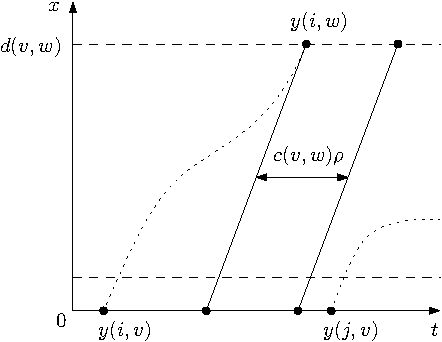
\includegraphics[width=0.8\textwidth]{figures/capacity_constraint.pdf}
  \caption{Illustration of the buffer constraint between $y(i, w)$ and
    $y(j, v)$. The slope of the two parallel lines is $v_{\max}$. The two dotted
    lines are examples of trajectories $x_{i}(t)$ and $x_{j}(t)$.}\label{fig:constraint}
\end{figure}

\begin{remark}
  The condition in Proposition~\ref{prop:buffer_constraint} is not always necessary. There are situations
  in which vehicle $j$ is able to cross $v$ earlier.
\end{remark}


\subsection*{Network scheduling}

We will now show how the trajectory optimization problem can be transformed into
a crossing time scheduling problem. We first introduce the notation that is used
to capture how vehicles drive through a network. After we show how the
MotionSynthesize procedure can be extended to networks, we present the general
form of the crossing time scheduling problem.

For each vehicle $i = (l,k)$, we will refer to $l$ as the \textit{vehicle
  class}, because vehicles are no longer bound to a unique lane.
%
We define a graph $(V,E)$ with \textit{labeled edges} as follows. Let $V$ denote
the indices of the intersections. Let $E$ denote the set of ordered triples
$(l, v, w)$ for each class $l$ whose vehicles travel from intersection $v$ to
$w$.
%
Let $d(v, w)$ denote the distance between intersections $v$ and $w$ and let
$c(v, w)$ denote the resulting capacity as given by
equation~\eqref{eq:max_capacity}. Let $\mathcal{N}(l)$ denote all the vehicles
of class $l$. Let $\mathcal{R}(l)$ denote the sequence of intersections visited
by vehicles from class $l$ and let $v_{0}(l)$ denote the first intersection on
this route.

Recall that trajectories for the single intersection problem can be generated by
the \texttt{MotionSynthesize} procedure, which is based on solving a linear
program.
%\begin{align*}
%  \texttt{MotionSynthesize}(z_{i,k}(t'_{0}), t'_{0}, t'_{f}, y) := \\
%  \text{arg min}_{x : [t'_{0}, t'_{f}] \rightarrow \mathbb{R}} \; &\int_{t_{0}}^{t_{f}} |x(t)|dt \\
%  \text{ subject to } \; & \ddot{x}(t) = u(t) , \text{ for all } t \in [t'_{0}, t'_{f}] ; \\
%  & 0 \leq \dot{x}(t) \leq v_{m} , \text{ for all } t \in [t'_{0}, t'_{f}] ; \\
%  & |u(t)| \leq a_{m} , \text{ for all } t \in [t'_{0}, t'_{f}] ; \\
%  & |x(t) - y(t)| \geq l , \text{ for all } t \in [t'_{0}, t'_{f}] ; \\
%  & x(t'_{0}) = x_{i,k}(t'_{0}); \quad \dot{x}(t'_{0}) = \dot{x}_{i,k}(t'_{0}) ; \\
%  & x(t'_{f}) = 0; \quad \dot{x}(t'_{f}) = v_{m} ,
%\end{align*}
%
%where initial state $z_{i,k}(t'_{0}) = (x_{i,k}(t'_{0}), \dot{x}_{i,k}(t'_{0}))$.
%
We present a natural extension of this procedure such that it can be used when a
vehicle encounters multiple intersections along its route. For vehicles from
class $l$, consider the sequence of checkpoints
%
\begin{align*}
  \tau = ((t_{0}, x_{0}), \dots, (t_{m}, x_{m})) ,
\end{align*}
where $t_{n}$ is a crossing time and $x_{n}$ is the position of the $n$th
intersection on $\mathcal{R}(l)$, relative to the first intersection.
%
Given the trajectory $y$ of the vehicle ahead, the trajectory for a vehicle with
checkpoint sequence $\tau$ is computed by the procedure
%
\begin{align*}
  \texttt{CheckpointTrajectory}(\tau, y) := \\
  \text{arg min}_{x : [t_{0}, t_{m}] \rightarrow \mathbb{R}} \; &\int_{t_{0}}^{t_{m}} |x(t)|dt \\
  \text{ subject to } \; & \ddot{x}(t) = u(t) ,& \text{ for all } t \in [t_{0}, t_{m}] , \\
  & 0 \leq \dot{x}(t) \leq v_{\max} ,& \text{ for all } t \in [t_{0}, t_{m}] , \\
  & |u(t)| \leq a_{\max} ,& \text{ for all } t \in [t_{0}, t_{m}] , \\
  & |x(t) - y(t)| \geq L ,& \text{ for all } t \in [t_{0}, t_{m}] , \\
  & x(t_{n}) = x_{n} ,& \text{ for all } n = 0, \dots, m , \\
  & \dot{x}(t_{n}) = v_{\max} ,& \text{ for all } n = 0, \dots, m .
\end{align*}

%Recall the single intersection scheduling model
%\begin{align*}
%  \min_{y} \quad & \sum_{i \in \mathcal{N}} y_{i} & \\
%  \text{s.t.} \quad & r_{i} \leq y_{i} & \text{ for } i \in \mathcal{N} , \\
%  & y_{i} + \rho_{i} \leq y_{j} & \text{ for } (i,j) \in \mathcal{C} , \\
%  & y_{i} + \sigma_{i} \leq y_{j} \text{ or } y_{j} + \sigma_{j} \leq y_{i} & \text{ for } \{i,j\} \in \mathcal{D} ,
%\end{align*}
%where we had
%\begin{align*}
%  \mathcal{D} &= \{ (i,j) \in \mathcal{N} : l(i) \neq l(j) \} , \\
%  \mathcal{C} &= \{ (i,j) \in \mathcal{N} : l(i) = l(j) , \, k(i) + 1 = k(j) \} .
%\end{align*}

From now on, we will assume $v_{\max} = 1$, without loss of generality. We
assume that vehicle arrive to the network at full speed and are \textit{safe} by
requiring that $r_{i} + L \leq r_{j}$ for every conjunctive pair
$(i, j) \in \mathcal{C}$. Furthermore, in order to keep the presentation of the
scheduling problem simple, we make the following assumption on vehicles routes.
\begin{assump}[Edge-Disjoint Routes]\label{assump:edge_disjoint_routes}
  Every lane $(v,w)$ is visited by at most one vehicle class. Formally,
  $(l_{1},v,w) \in E$ and $(l_{2},v,w) \in E$ implies $l_{1}=l_{2}$.
\end{assump}

We now show how to obtain schedules in this model by formulating a MILP. Let
$y(i,v)$ denote the crossing time of vehicle $i$ at intersection $v \in V$. Let
$\mathcal{C}$ be the conjunctive pairs and let $\mathcal{D}^{v}$ denote the
disjunctive pairs at intersection $v \in V$.
%
Writing $\texttt{conj(\dots)}$ and $\texttt{disj}(\dots)$ for the usual conjunctive and disjunctive
constraints, we propose to solve the optimization problem
\begin{subequations}\label{eq:network_problem}
\begin{align}
  \min_{y} \quad & \sum_{i \in \mathcal{N}} \sum_{v \in \mathcal{R}(l(i))} y(i,v) & \\
  \text{s.t.} \quad & r_{i} \leq y(i, v_{0}(l(i))) & \text{ for } i \in \mathcal{N} , \\
  & \texttt{conj}(y(i,v), y(j,v)) & \text{ for } (i,j) \in \mathcal{C}, v \in V , \\
  & \texttt{disj}(y(i,v), y(j,v)) & \text{ for } \{i,j\} \in \mathcal{D}^{v}, v \in V , \\
  & y(i, v) + d(v, w) \leq y(i, w) & \text{ for } i \in \mathcal{N}(l), (l, v, w) \in E, \label{eq:travel_delay} \\
  & y(i, w) + \rho(v, w) \leq y(j, v) & \text{ for } (i,j,v,w) \in \mathcal{F} , \label{eq:buffer_constraints}
\end{align}
\end{subequations}
where $\mathcal{F}$ is defined as
\begin{align*}
  \mathcal{F} = \{ (i,j,v,w) : i,j \in \mathcal{N}(l), k(i) + c(v,w) = k(j),  (l,v,w) \in E\}
\end{align*}
and we have $\rho(v, w) = c(v, w) L - d(v, w)$ from Proposition~\ref{prop:buffer_constraint}. Each
$(i,j,v,w) \in \mathcal{F}$ represents a pair of vehicles driving on the same lane
$(v,w)$, for which the first vehicle must have made enough space in the lane
before vehicle $j$ can enter.
%
%
%Under Assumption~\ref{assump:edge_disjoint_routes}, the constraints~\eqref{eq:buffer_constraints} yield the
%following property of schedules (c.f. Theorem 4.1 in~\cite{heitmannJobshopSchedulingLimited2007} or Theorem 1 in~\cite{bruckerJobshopSchedulingLimited2006}).
%
%\begin{proposition}
%  Let $y$ be a solution to the network scheduling problem~\eqref{eq:network_problem} with
%  Assumption~\ref{assump:edge_disjoint_routes}. For each $(l,v,w) \in E$, there are always at most $b(v,w)$
%  vehicles at lane $(v,w)$.
%\end{proposition}
%\begin{proof}
%  Let $i$ be a vehicle that has $(v,w)$ on its route. Define the occupancy
%  interval $D_{i} = [y(i,v), \, y(i,w)]$, then we say that $i$ occupies $(v,w)$
%  at some time $t$ whenever $t \in D_{i}$.
%  %
%  Therefore, the number of vehicles in $(v,w)$ at time $t$ equals the number of such
%  intervals containing $t$.
%
%  Suppose we have a schedule $y$ such that at some time $t$, there are strictly
%  more than $b(v,w)$ vehicles $i$ such that $t \in D_{i}$.
%  %
%  Let $i_{1}$ be such that $y(i_{1},v) \leq y(i,v)$ for all $i$ such that $t \in D_{i}$.
%  From the conjunctive constraints at $v$ follows that there is some $n$ such that
%  \begin{align*}
%    y(i_{1}, v) + \rho_{i_{1}} \leq y(i_{2}, v) + \rho_{i_{2}} \leq \dots \leq y(i_{n}, v) + \rho_{i_{n}} ,
%  \end{align*}
%  where $i_{k} = (l(i_{1}), k(i_{1}) + k - 1)$.
%  %
%  By Assumption~\ref{assump:edge_disjoint_routes}, the only vehicles that can enter $(v,w)$ after
%  $i_{1}$ are precisely $i_{2}, \dots, i_{n}$. By assumption, we have $n \geq b(v,w) + 1$,
%  so $j = (l(i_{1}), k(i_{1}) + b(v,w)) \in \{i_{2}, \dots, i_{n}\}$ is such
%  that $t \in D_{j}$.
%  Hence, $y(j,v) \leq t \leq y(i,w)$,
%  which violates constraint~\eqref{eq:buffer_constraints}
%  and thus contradicts the feasibility of $y$.
%\end{proof}

\subsection*{Overlapping routes}

In problem~\ref{eq:network_problem}, note that the conjunctions $\mathcal{C}$
did not depend on the intersection like the disjunctions, because the
conjunctive ``chains'' stays the same along the route. Whenever we drop
Assumption~\ref{assump:edge_disjoint_routes}, it becomes possible for vehicles from different
classes to merge onto the same lane. Once one the same lane, they also need to
maintain their relative order, so conjunctive constraints need to be introduced
depending on which disjunctive decisions were made at an upstream intersection.

Note that the formulation of the capacity constraints~\eqref{eq:buffer_constraints} hinges on the chains
of conjunctive arcs in the disjunctive graph. In other words, the pairs of
vehicles involved in these ``delayed conjunctive constraints'' does not depend
on the ordering of vehicles at intersections. Once we drop Assumption~\ref{assump:edge_disjoint_routes}, these
delayed constraints can also appear among vehicles from different routes,
depending on their ordering. In principle, it is possible to add these
conditional constraints to the MILP. However, we expect that even encoding all
of them requires too much computing time and memory.


\subsection*{Related scheduling problems}

We now show that the above problem can be interpreted as a variation of the
classical job-shop scheduling problem (JSSP) with setup-times. Intersections
play the role of machines and each vehicle is modeled by a job, whose operations
correspond to crossing the intersections along its route. The following three
aspects distinguish the current problem from classical JSSP.

First of all, we assume that vehicles cannot overtake other vehicles on the same
lane, so the order in which vehicles arrive to a lane needs to be maintained at
all downstream intersections. This introduces a set of additional precedence
constraints that are not required in general JSSP.

Furthermore, note that constraints~\eqref{eq:travel_delay} model travel delays between
intersections. For some networks, the problem can be transformed back to JSSP
without travel delays by an appropriate time shifting procedure. In the general
case, such a transformation is also possible by introducing additional machines
that explicitly model the \textit{travel operation}. Such travel delays have been studied
before in a model where a fleet of autonomous vehicles moves operations between
a set of machines~\cite{berterottiereFlexibleJobshopScheduling2024}.

The third extensions involves the limited buffer size at machines, which has
been considered before~\cite{heitmannJobshopSchedulingLimited2007}. With these
kind of constraints, the problem becomes stricly more general than JSSP.


\subsection*{Constructive neural heuristic}

Like we did for the single intersection, we are now going to define heuristics
in terms of choosing which vehicle may cross next on which intersection.
%
Again, we model this process as a deterministic finite-state automaton, with
input alphabet given by
\begin{align*}
  \Sigma = \{ (l,v) : l \in \{1, \dots, n\} , v \in V \} ,
\end{align*}
where $n$ is the number of classes.
%
Let $v \in V$ be some intersection, then $\pi(v)$ denotes the local crossing
order of intersection $v$, analogously to $\pi$ in the single intersection case.
%
Let $s$ be an instance of network problem~\eqref{eq:network_problem}, then the
state $(s, \pi)$ encodes the local crossing order $\pi(v)$ for each intersection
$v$.
%
Let $n(l, v)$ denote the number of scheduled vehicles from class $l$ at
intersection $v$.
%
Every action $(l, v)$ is a pair of a class $l$ and some intersection
$v \in \mathcal{R}(l)$ and corresponds to appending the next unscheduled vehicle
from class $l$ to the local ordering $\pi(v)$.

We keep track of the lower bounds $\mathrm{LB}_{\pi}(i, v)$ for every
vehicle-intersection pair, where $\pi$ denotes the current global (partial)
ordering, consisting of the collection of all local orderings
$\{ \pi(v) : v \in V \}$.
%
Because all constraints are of the form
\begin{align*}
  y(i, v) + \alpha(i, v, j, w) \leq y(j, w) ,
\end{align*}
they can be thought of as arcs with weight $\alpha(i, v, j, w)$ in the
disjunctive graph, which has a node for every vehicle-intersection pair
$(i, v)$. In this way, the lower bounds are simply defined as
\begin{align*}
  \mathrm{LB}_{\pi}(i, v) = \max_{(j, w) \in N_{\pi}^{-}(i, v)} \mathrm{LB}_{\pi}(j, w) + \alpha(i, v, j, w).
\end{align*}
%
As in the single intersection problem, a complete ordering $\pi$ provides us
with a crossing time schedule $y(i, v) = \mathrm{LB}_{\pi}(i, v)$. For every
(partial) ordering $\pi$, the lower bounds can simply be computed by solving a
linear program. Alternatively, the structure of the disjunctive graph can be
used for a more direct calculation, as we show next.

\begin{proposition}
  The empty schedule $\pi = \varnothing$ has lower bounds
  \begin{align}
    \mathrm{LB}_{\varnothing}(i, v) = r_{i} + d(v_{0}(l(i)), v) .
  \end{align}
\end{proposition}
\begin{proof}
  Since there are no disjunctive constraints in $G(\varnothing)$, we can
  consider each class $l$ separately.
  %
  Because we assumed that $r_{i} + L \leq r_{j}$ for every
  $(i, j) \in \mathcal{C}$, the conjunctive constraints at $v_{0}(l)$ must hold.
  Furthermore all travel constraints are tight in this definition of
  $\mathrm{LB}_{\varnothing}$.
  %
  We show that conjunctive constraints at downstream intersections are satisfied
  by induction on $v \in \mathcal{R}(l)$. Let $(i, j) \in \mathcal{C}$ and let
  $(v, w)$ be an edge of route $\mathcal{R}(l)$, then
  \begin{align*} \mathrm{LB}_{\varnothing}(i, w) + L = \mathrm{LB}_{\varnothing}(i, v) + d(v, w) + L \leq \mathrm{LB}_{\varnothing}(j, v) + d(v, w) = \mathrm{LB}_{\varnothing}(j, w) .
  \end{align*}
  %
  It remains to show that all buffer constraints are satisfied. Consider a pair
  of vehicles $i = (l, k)$ and $j = (l, k + c(v,w))$. By the chain of
  conjunctive constraints between $i$ and $j$, we have
  \begin{align*}
    \mathrm{LB}_{\varnothing}(i, v) + c(v, w) L \leq \mathrm{LB}_{\varnothing}(j, v) .
  \end{align*}
  From the travel constraints, we have
  \begin{align*}
    \mathrm{LB}_{\varnothing}(i, w) - d(v,w) = \mathrm{LB}_{\varnothing}(i, v) .
  \end{align*}
  Together, these two equations imply the buffer constraint
  \begin{equation*}
    \mathrm{LB}_{\varnothing}(i, w) + c(v, w) L - d(v, w) \leq
    \mathrm{LB}_{\varnothing}(j, v) . \qedhere
  \end{equation*}
\end{proof}

Starting from $\mathrm{LB}_{\varnothing}$, we update the lower bounds every time
a new vehicle is added to $\pi$. Often, only a subset of the lower bounds is
affected, so we propagate only the necessary changes through the disjunctive
graph. For $i = (l, k) \in \mathcal{N}(l)$, let $\mathrm{next}(i) = (l, k + 1)$
denote its successor in the conjunctive chain, if it exists. Similarly, we use
the notation $\mathrm{prev}(v)$ and $\mathrm{next}(v)$ for the previous and next
intersection, respectively, on the route $\mathcal{R}(l)$, if they exist. We
write the assignment operation $x \xleftarrow{\max} y$ as a shorthand for
$x \gets \max(x, y)$.

\begin{proposition}
  Algorithm~\ref{alg:LB_update} maintains the correct values of $LB_{\pi}$
  whenever some vehicle $i$ is added to local ordering $\pi(v)$.
\end{proposition}
\begin{proof}
  For all lower bounds involving $l(i)$, nothing changes.
  For each class at $v$ other than $l(i)$, we process the disjunctive arc
  towards the next unscheduled vehicle $j$ by setting
  \begin{align*}
    \mathrm{LB}_{\pi}(j, v) \xleftarrow{\max} \mathrm{LB}(i, v) + \sigma .
  \end{align*}
  %
  Then for each $l(j)$ of these other classes, we propagate the changes through
  the disjunctive graph as follows.
\end{proof}


\begin{algorithm}
  \caption{Update $\mathrm{LB}_{\pi}$ after vehicle $i$ is added to $\pi(v)$, by
    propagating changes over the disjunctive graph, under
    Assumption~\ref{assump:edge_disjoint_routes}.}\label{alg:LB_update}
\begin{algorithmic}[1]
\end{algorithmic}
\end{algorithm}

% \For{each vehicle class $l$}
%   \For{$w \in \mathcal{R}(l)$ in sequence order}
%     \State $v \gets$ predecessor of $w$ on route $\mathcal{R}(l)$
%     \If{$v$ exists}

%       \For{$j \in \mathcal{N}(l)$ in order of ascending arrival time}
%         \State $\mathrm{LB}_{\pi}(j, w) \xleftarrow{\max} \mathrm{LB}_{\pi}(j, v) + d(v, w)$ \Comment{travel constraints}

%         \State $k \gets k(j) - c(v, w)$
%         \If{$k > 0$}
%           \State $i \gets (l, k)$ \Comment{ s.t. $(i,j,v,w) \in \mathcal{F}$ }
%           \State $\mathrm{LB}_{\pi}(j, v) \xleftarrow{\max} \mathrm{LB}_{\pi}(i, w) + \rho(v, w)$ \Comment{buffer constraints}
%         \EndIf
%       \EndFor

%     \EndIf

%     \For{all consecutive vehicle $i \rightarrow j$ of class $l$}
%       \State $\mathrm{LB}_{\pi}(j, w) \xleftarrow{\max} \mathrm{LB}_{\pi}(i, w) + \rho$ \Comment{conjunctions}
%     \EndFor
%   \EndFor
% \EndFor





%\begin{align*}
% r_{i} &\leq \text{LB}_{\pi}(i, v) \text{ release, } \\
%  \text{LB}_{\pi}(i, v) + w(i, j) &\leq \text{LB}_{\pi}(j, v) \text{ local precedence } i \rightarrow j \\
%  \text{LB}_{\pi}(i, v) + d(v, w)    &\leq  \text{LB}_{\pi}(i, w)   \text{ travel, } \\
%  \text{LB}_{\pi}(i, w) + \rho(v, w) &\leq  \text{LB}_{\pi}(j, v) \text{ buffer } (i,j,v,w) \in \mathcal{F} ,  \\
%\end{align*}

\newpage

\subsubsection*{Parameterization}

Show how to build a suitable embedding of the current state, based on lower
bounds $\mathrm{LB}_{\pi}$.

\section*{Traffic as job-shop scheduling}

The Job-Shop Scheduling Problem (JSSP) is a widely studied problem in which a
set of $n$ jobs must be assigned to non-overlapping time slots on a set of $m$
machines. Each job $i$ has a set of $n_{i}$ operations
$O_{i1}, \dots, O_{in_{i}}$ that need to be executed in this order. Each
operation $O_{ij}$ requires $p_{ij}$ processing time on machine $M_{ij}$. Each
machine can process at most one operation and early preemption is not allowed.
The task of the scheduler is to determine a valid schedule of start times
$y_{ij}$ for each operation, while minimizing some objective function. Let
$C_{ij} = y_{ij} + p_{ij}$ denote the \textit{completion time} of operation
$O_{ij}$, then the \textit{makespan} objective is given by the latest completion
time
\begin{align*}
  \max_{i,j} C_{ij} .
\end{align*}
Another objective is the \textit{total completion time}, given by
\begin{align*}
  \sum_{i=1}^{n} \sum_{j=1}^{m} C_{ij} ,
\end{align*}
which may be intuitively thought of as representing some sort of total cost of
inventory, assuming we need to physically store jobs somewhere.

A commonly used representation of JSSP instances is the \textit{disjunctive
  graph} $G = (\mathcal{O}, \mathcal{C}, \mathcal{D})$, with vertices
$\mathcal{O} = \{ O_{ik} : 1 \leq i \leq n, 1 \leq k \leq n_{i} \}$
corresponding all the operations. The set of \textit{conjunctive arcs}
$\mathcal{C}$ encodes all the precedence constraints
$O_{i,k} \rightarrow O_{i,k+1} $ among each job's operations. The set of
\textit{disjunctive edges} $\mathcal{D}$ consists of undirected edges between
each pair of operations from distinct jobs that need to be processed on the same
machine, effectively encoding all such \textit{conflicts}. Each valid schedule
induces an ordering of operations on machines that is encoded by fixing the
direction of each disjunctive edge such that we obtain a direct acyclic graph.

% discuss modeling of buffers

\newpage
\section*{Implementation details}

We set the capacity of each lane according to equation~\eqref{eq:max_capacity},
except for lanes from an entry point. These so-called \textit{entry lanes} have
unlimited capacity, which allows us to specify any kind of arrival time pattern.

\begin{figure}
  \centering
  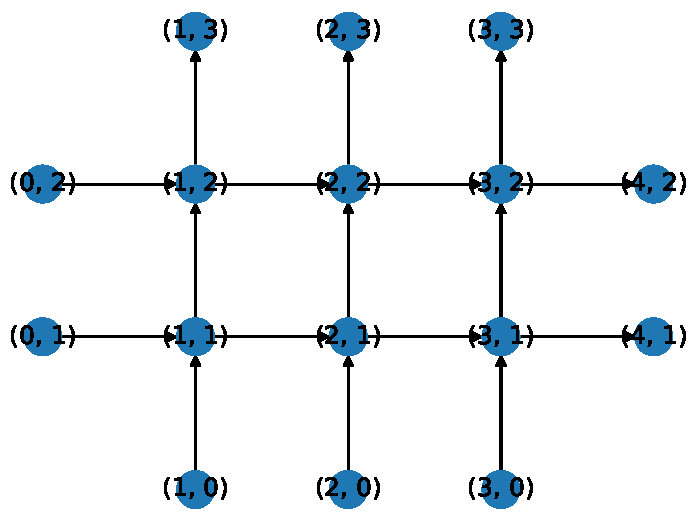
\includegraphics[width=0.7\textwidth]{figures/network_graph_example.pdf}
  \caption{Example of connectivity graph of traffic network.}
\end{figure}


\bibliography{references}
\bibliographystyle{ieeetr}

\end{document}
